\documentclass[12pt]{beamer}

\usetheme[white,sections]{Wisconsin}
\usepackage{fancyvrb}
\usepackage{color}
\usepackage[normalem]{ulem}
\usepackage{xcolor}
\usepackage{anyfontsize}
\usepackage{wrapfig}
\usepackage{graphicx}

\usepackage{tikz}
\usetikzlibrary{shapes.arrows}
\tikzset{
    myarrow/.style={
        draw,
        fill=orange,
        single arrow,
        minimum height=4.5ex,
        single arrow head extend=1ex
    }
}
\tikzset{
    mydoublearrow/.style={
        draw,
        fill=orange,
        double arrow,
        minimum height=10.5ex,
        single arrow head extend=1ex
    }
}

\newcommand{\arrowup}{%
\tikz [baseline=-0.5ex]{\node [myarrow,rotate=90] {};}
}
\newcommand{\arrowdown}{%
\tikz [baseline=-1ex]{\node [myarrow,rotate=-90] {};}
}
\newcommand{\doublearrow}{%
\tikz [baseline=-1ex]{\node [mydoublearrow,rotate=0] {};}
}

\begin{document}
\newcommand*{\alphabet}{ABCDEFGHIJKLMNOPQRSTUVWXYZabcdefghijklmnopqrstuvwxyz}
\newlength{\highlightheight}
\newlength{\highlightdepth}
\newlength{\highlightmargin}
\setlength{\highlightmargin}{2pt}
\settoheight{\highlightheight}{\alphabet}
\settodepth{\highlightdepth}{\alphabet}
\addtolength{\highlightheight}{\highlightmargin}
\addtolength{\highlightdepth}{\highlightmargin}
\addtolength{\highlightheight}{\highlightdepth}
\setbeamertemplate{bibliography entry title}{}
\setbeamertemplate{bibliography entry location}{}
\setbeamertemplate{bibliography entry note}{}
\newcommand*{\Highlight}{\rlap{\textcolor{HighlightBackground}{\rule[-\highlightdepth]{\linewidth}{\highlightheight}}}}
\setbeamertemplate{bibliography item}[text]
\setbeamercolor{section in toc}{fg=white}
\setbeamercolor{bibliography entry author}{fg=black}
\setbeamercolor{bibliography item}{fg=black}
\setbeamercolor*{bibliography entry title}{fg=black}
%\setbeamerfont{section number projected}{size=\tiny}
\setbeamerfont{section number projected}{size=\fontsize{6}{6}\selectfont}
\setbeamercolor{section number projected}{bg=UWRed,fg=white}
\hypersetup{linkcolor=white,urlcolor=white}

\AtBeginSection{\frame{\sectionpage}}
\defbeamertemplate{section page}{mine}[1][]{%
  \begin{centering}
    {\usebeamerfont{section name}\usebeamercolor[fg]{section name}#1}
    \vskip1em\par
    \begin{beamercolorbox}[sep=12pt,center]{part title}
      \usebeamerfont{section title}\insertsection\par
    \end{beamercolorbox}
  \end{centering}
}
\setbeamertemplate{section page}[mine]

%%%%%%%%%%%%%%%%%%%%%%%%%%%%%%%%%%%%%%%%%%%%%%%%%%%%%%%%%%%%%%%%%%%%%%%%%%%%%%%%
\title{Quality Assurance within the PyNE Open Source Toolkit}   
\author{Elliott Biondo$^1$, Anthony Scopatz$^1$, Matthew Gidden$^1$, \\ 
        Rachel Slaybaugh$^2$, Cameron Bates$^2$, Paul P.H. Wilson$^1$}
\institute{$^1$University of Wisconsin - Madison \\ 
           $^2$University of California, Berkeley}
\date{Nov. 11, 2014}
\frame[plain]{\titlepage \addtocounter{framenumber}{-1}} 

%%%%%%%%%%%%%%%%%%%%%%%%%%%%%%%%%%%%%%%%%%%%%%%%%%%%%%%%%%%%%%%%%%%%%%%%%%%%%%%%
%%%%%%%%%%%%%%%%%%%%%%%%%%%%%%%%%%%%%%%%%%%%%%%%%%%%%%%%%%%%%%%%%%%%%%%%%%%%%%%%
%%%%%%%%%%%%%%%%%%%%%%%%%%%%%%%%%%%%%%%%%%%%%%%%%%%%%%%%%%%%%%%%%%%%%%%%%%%%%%%%
\section{Background}
%%%%%%%%%%%%%%%%%%%%%%%%%%%%%%%%%%%%%%%%%%%%%%%%%%%%%%%%%%%%%%%%%%%%%%%%%%%%%%%%
%%%%%%%%%%%%%%%%%%%%%%%%%%%%%%%%%%%%%%%%%%%%%%%%%%%%%%%%%%%%%%%%%%%%%%%%%%%%%%%%
%%%%%%%%%%%%%%%%%%%%%%%%%%%%%%%%%%%%%%%%%%%%%%%%%%%%%%%%%%%%%%%%%%%%%%%%%%%%%%%%
\begin{frame}[fragile]
\frametitle{The PyNE Toolkit}

Trans-institutional, open source project
Nuclear Science and engineering analysis and similations

27 contributors, 21 with over 1000 lines of code/tests/documentation.
Top 20 "trending 
Common Python iterface
In the top 25 "trending" C++ repositories on GitHub.com

\end{frame}
%%%%%%%%%%%%%%%%%%%%%%%%%%%%%%%%%%%%%%%%%%%%%%%%%%%%%%%%%%%%%%%%%%%%%%%%%%%%%%%%
\begin{frame}[fragile]
\frametitle{The PyNE Toolkit}

\end{frame}
%%%%%%%%%%%%%%%%%%%%%%%%%%%%%%%%%%%%%%%%%%%%%%%%%%%%%%%%%%%%%%%%%%%%%%%%%%%%%%%%
\begin{frame}
\frametitle{My work within PyNE}

\end{frame}
%%%%%%%%%%%%%%%%%%%%%%%%%%%%%%%%%%%%%%%%%%%%%%%%%%%%%%%%%%%%%%%%%%%%%%%%%%%%%%%%
\begin{frame}[fragile]
\frametitle{Quality assurance}

\end{frame}
%%%%%%%%%%%%%%%%%%%%%%%%%%%%%%%%%%%%%%%%%%%%%%%%%%%%%%%%%%%%%%%%%%%%%%%%%%%%%%%%
\begin{frame}[fragile]
\frametitle{Quality assurance for nuclear engineering}

\begin{columns}[T]
\begin{column}{0.5\textwidth}

\includegraphics[width=\textwidth]{figures/nqa-1-2008.png}
\end{column}
\begin{column}{0.5\textwidth}
The NRC \cite{NRC} endorses the American Society of Mechical Engineers (ASME)
NQA-1-2008 standard with the NQA-1a-2008 addenum for the licensing of power
plants and reprocessing facilities.
\end{column}
\end{columns}


\end{frame}
%%%%%%%%%%%%%%%%%%%%%%%%%%%%%%%%%%%%%%%%%%%%%%%%%%%%%%%%%%%%%%%%%%%%%%%%%%%%%%%%
\begin{frame}[fragile]
\frametitle{Motivation}

\end{frame}


%%%%%%%%%%%%%%%%%%%%%%%%%%%%%%%%%%%%%%%%%%%%%%%%%%%%%%%%%%%%%%%%%%%%%%%%%%%%%%%%
%%%%%%%%%%%%%%%%%%%%%%%%%%%%%%%%%%%%%%%%%%%%%%%%%%%%%%%%%%%%%%%%%%%%%%%%%%%%%%%%
%%%%%%%%%%%%%%%%%%%%%%%%%%%%%%%%%%%%%%%%%%%%%%%%%%%%%%%%%%%%%%%%%%%%%%%%%%%%%%%%
\section{NQA-1 Standards}
%%%%%%%%%%%%%%%%%%%%%%%%%%%%%%%%%%%%%%%%%%%%%%%%%%%%%%%%%%%%%%%%%%%%%%%%%%%%%%%%
%%%%%%%%%%%%%%%%%%%%%%%%%%%%%%%%%%%%%%%%%%%%%%%%%%%%%%%%%%%%%%%%%%%%%%%%%%%%%%%%
%%%%%%%%%%%%%%%%%%%%%%%%%%%%%%%%%%%%%%%%%%%%%%%%%%%%%%%%%%%%%%%%%%%%%%%%%%%%%%%%

\begin{frame}[fragile]
\frametitle{The Waterfall method}
\centerline{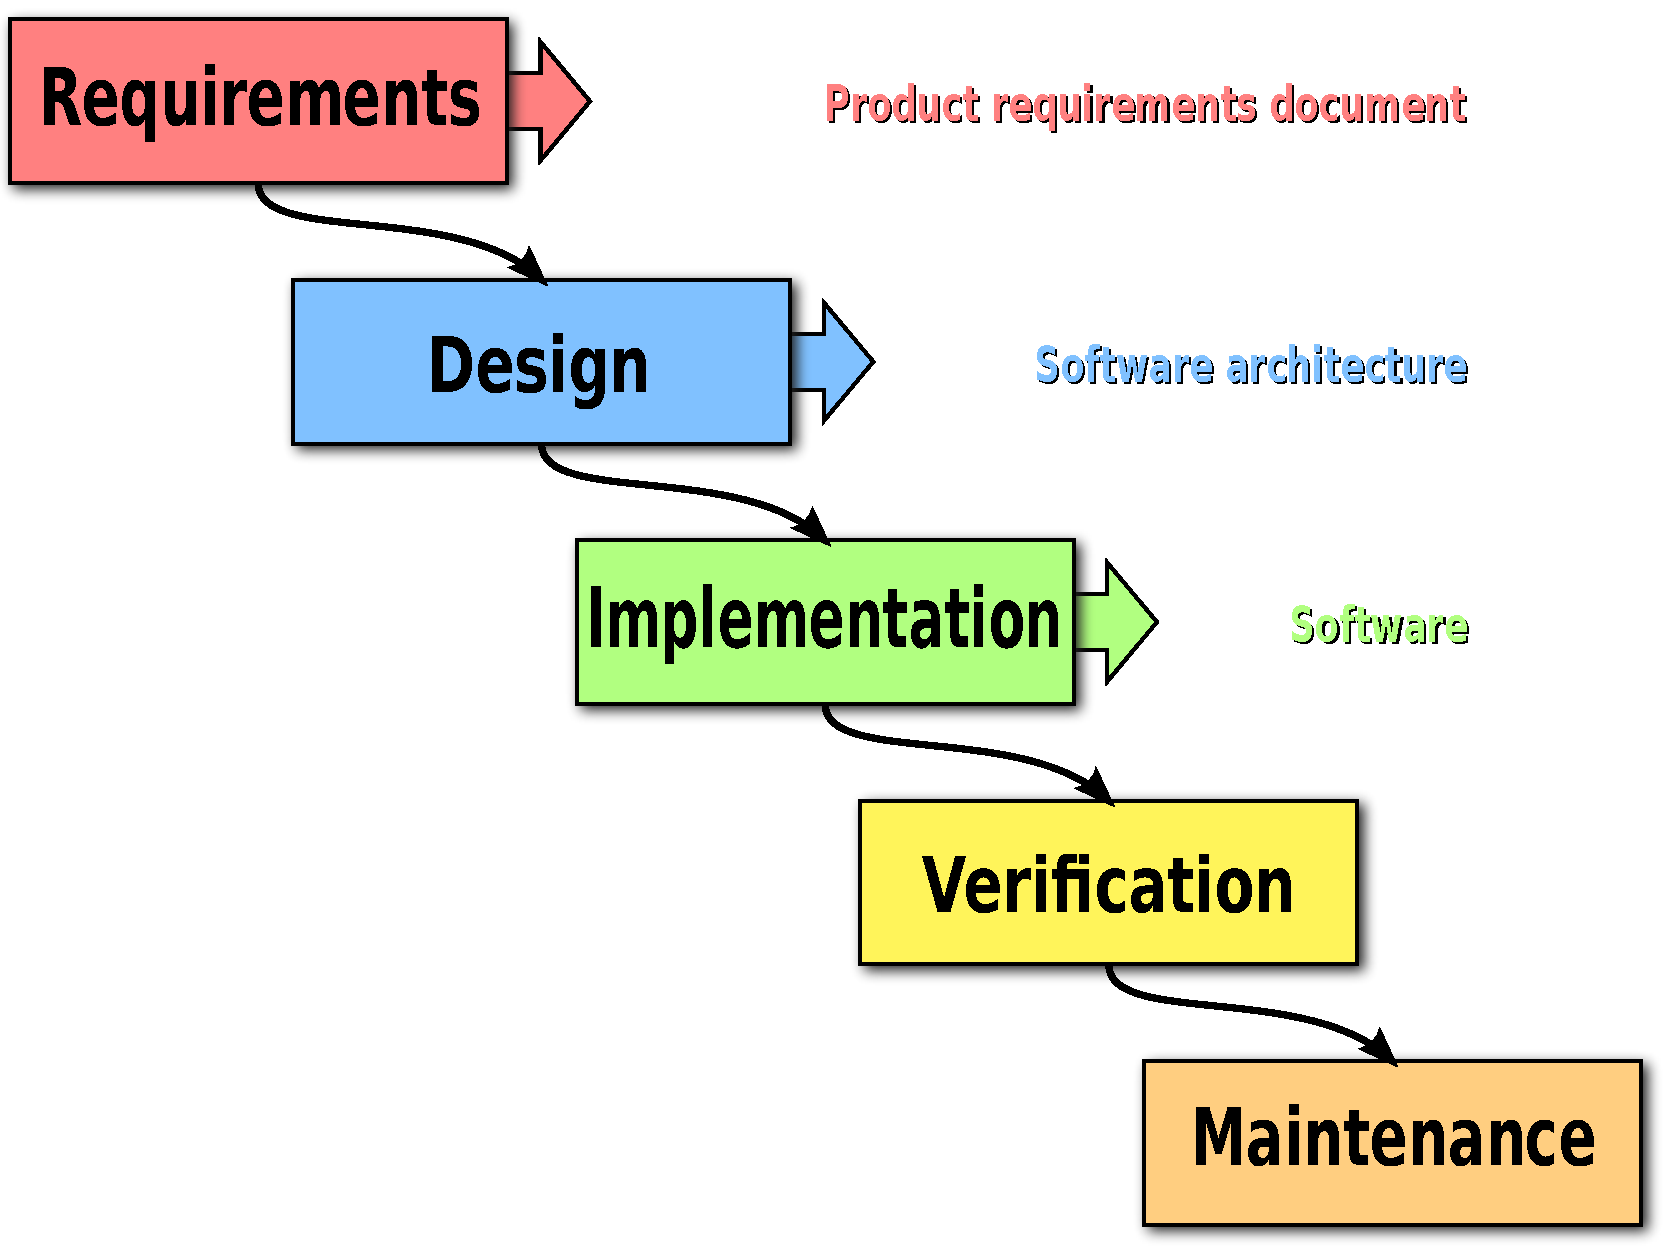
\includegraphics[width=0.8\textwidth]{figures/waterfall.pdf}}
Figure from \cite{waterfall_wiki}
\end{frame}


%%%%%%%%%%%%%%%%%%%%%%%%%%%%%%%%%%%%%%%%%%%%%%%%%%%%%%%%%%%%%%%%%%%%%%%%%%%%%%%%
\begin{frame}
\frametitle{The gist}

\begin{itemize}
\item{Use the Water Method}
\item{Document every step}
\end{itemize}

\end{frame}

%%%%%%%%%%%%%%%%%%%%%%%%%%%%%%%%%%%%%%%%%%%%%%%%%%%%%%%%%%%%%%%%%%%%%%%%%%%%%%%%
\begin{frame}
\frametitle{More concrete requirements}


\end{frame}
%%%%%%%%%%%%%%%%%%%%%%%%%%%%%%%%%%%%%%%%%%%%%%%%%%%%%%%%%%%%%%%%%%%%%%%%%%%%%%%%



%%%%%%%%%%%%%%%%%%%%%%%%%%%%%%%%%%%%%%%%%%%%%%%%%%%%%%%%%%%%%%%%%%%%%%%%%%%%%%%%
\section{QA within PyNE}

\begin{frame}
\frametitle{Applicability of NQA-1}

\end{frame}


\begin{frame}[fragile]
\frametitle{Challenges}

\begin{itemize}
\item{PyNE developer are a diverse bunch}:
   \begin{itemize}
   \item{Undergraduates through tenured profesors.}
   \item{Varying levels of software development experience.}
   \item{Spare time vs. funded work.}
   \item{Research vs. production level.}
   \end{itemize}
\item{Agile Software Development}
\end{itemize}

\end{frame}


\begin{frame}
\frametitle{Version Control}
\end{frame}

\begin{frame}
\frametitle{Pull Requests}
\end{frame}

\begin{frame}
\frametitle{Requirements for Pull Requests}
In order to be accepted:

\end{frame}



\begin{frame}
\frametitle{Continuous Integration}
\end{frame}


\begin{frame}
\frametitle{The PyNE QA standard}
Everything heretofor has been the bare minimum to be accpeted into PyNE
\end{frame}


\begin{frame}
\frametitle{Work to date}

Ratified Quality Assurance
One module fully complaint
Major topic at the PyNE 3 day Hack-a-ton at Berkeley this weekend.

\end{frame}




\begin{frame}[fragile]
\frametitle{Acknowledgements}


\includegraphics[height=2cm]{figures/NRClogo.png} \\

\end{frame}

%%%%%%%%%%%%%%%%%%

%%%%%%%%%%%%%%%%%%%%%%%%%%%%%%%%%%%%%%%%%%%%%%%%%%%%%%%%%%%%%%%%%%%%%%%%%%%%%%%%
%%%%%%%%%%%%%%%%%%%%%%%%%%%%%%%%%%%%%%%%%%%%%%%%%%%%%%%%%%%%%%%%%%%%%%%%%%%%%%%%
%%%%%%%%%%%%%%%%%%%%%%%%%%%%%%%%%%%%%%%%%%%%%%%%%%%%%%%%%%%%%%%%%%%%%%%%%%%%%%%%
\section*{Questions?}
%%%%%%%%%%%%%%%%%%%%%%%%%%%%%%%%%%%%%%%%%%%%%%%%%%%%%%%%%%%%%%%%%%%%%%%%%%%%%%%%
%%%%%%%%%%%%%%%%%%%%%%%%%%%%%%%%%%%%%%%%%%%%%%%%%%%%%%%%%%%%%%%%%%%%%%%%%%%%%%%%
%%%%%%%%%%%%%%%%%%%%%%%%%%%%%%%%%%%%%%%%%%%%%%%%%%%%%%%%%%%%%%%%%%%%%%%%%%%%%%%%

%\begin{frame}[allowframebreaks]
\begin{frame}[plain]
        \tiny
        \frametitle{References}
        \bibliographystyle{ans}
        \color{black}
        \bibliography{refs}
\end{frame}

%%%%%%%%%%%%%%%%%%%%%%%%%%%%%%%%%%%%%%%%%%%%%%%%%%%%%%%%%%%%%%%%%%%%%%%%%%%%%%%%
%%%%%%%%%%%%%%%%%%%%%%%%%%%%%%%%%%%%%%%%%%%%%%%%%%%%%%%%%%%%%%%%%%%%%%%%%%%%%%%%
%%%%%%%%%%%%%%%%%%%%%%%%%%%%%%%%%%%%%%%%%%%%%%%%%%%%%%%%%%%%%%%%%%%%%%%%%%%%%%%%
\end{document}
%%%%%%%%%%%%%%%%%%%%%%%%%%%%%%%%%%%%%%%%%%%%%%%%%%%%%%%%%%%%%%%%%%%%%%%%%%%%%%%%
%%%%%%%%%%%%%%%%%%%%%%%%%%%%%%%%%%%%%%%%%%%%%%%%%%%%%%%%%%%%%%%%%%%%%%%%%%%%%%%%
